\newpage\setcounter{dang}{0}
\section*{BÀI TẬP CUỐI CHƯƠNG}
\subsection{BÀI TẬP TỰ LUẬN}
\setcounter{bt}{0}
\begin{bt}%[0H3Y1-1]
	Cho đường thẳng $d:\left\{\begin{array}{l}x=x_{0}+a t \\ y=y_{0}+b t\end{array}\right.$ ( $t$ là tham số) với $a, b$ không đồng thời bằng $0$.
	\begin{enumerate}[a)]
	\item Chỉ ra một vectơ chỉ phương của $d$.
	\item Chỉ ra một vectơ pháp tuyến của $d$.
	\item Chỉ ra một điểm có tọa độ khác $\left(x_{0} ; y_{0}\right)$ và thuộc đường thẳng $d$.
	\end{enumerate}
\loigiai{
	\begin{enumerate}[a)]
	\item Một vectơ chỉ phương của $d$ là $\overrightarrow{u}=(a;b)$.
	\item Một vectơ pháp tuyến của $d$ là $\overrightarrow{n}=(b;-a)$.
	\item Một điểm có tọa độ khác $\left(x_{0} ; y_{0}\right)$ và thuộc đường thẳng $d$ là $M(x_0+a;y_0+b)$ (chọn $t=1$).
	\end{enumerate}
	}
\end{bt}
\begin{bt}%[0H3Y1-1]
	Cho đường thẳng $d: a x+b y+c=0$ vối $a, b$ không đồng thời bằng $0$.
	\begin{enumerate}[a)]
	\item Chỉ ra một vectơ pháp tuyến của $d$.
	\item Chỉ ra một vectơ chỉ phương của $d$.
	\item Cho $a, b$ đều khác $0$. Chỉ ra một điểm thuộc đường thẳng $d$ mà không nằm trên cả hai trục toạ độ.
	\end{enumerate}
\loigiai{
	\begin{enumerate}[a)]
	\item Một vectơ pháp tuyến của $d$ là $\overrightarrow{u}=(a;b)$.
	\item Một vectơ chỉ phương của $d$ là $\overrightarrow{n}=(b;-a)$.
	\item Ta có nhận xét:\\
	\textbf{Nhận xét.} Điểm $\mathrm{A}$ thuộc đường thẳng $\Delta: a x+b y+c=0$ (ĐK: $a^{2}+b^{2} \neq 0$) có dạng $A\left(t ; \dfrac{-a t-c}{b}\right)$ với $b \neq 0$ hoặc $A\left(\dfrac{-b t-c}{a} ; t\right)$ với $a \neq 0$.\\
	\textbf{Áp dụng.} Một điểm thuộc đường thẳng $d$ mà không nằm trên cả hai trục toạ độ là $M\left(1; \dfrac{-a-c}{b}\right)$ với $t=1$.
	\end{enumerate}
	}
\end{bt}
\begin{bt}%[0H2B2-1]
	Trong mặt phẳng toạ độ $Oxy$, cho tam giác $MNP$ có $M(2 ; 1), N(-1 ; 3), P(4 ; 2)$.
	\begin{enumerate}[a)]
	\item Tìm toạ độ của các vectơ $\overrightarrow{O M}, \overrightarrow{M N}, \overrightarrow{M P}$;
	\item Tính tích vô hưởng $\overrightarrow{MN}.\overrightarrow{M P}$;
	\item Tính độ dài các đoạn thẳng $M N, M P$;
	\item Tính $\cos \widehat{N M P}$;
	\item Tìm tọa độ trung điểm $I$ của $N P$ và trọng tâm $G$ của tam giác $M N P$.
	\end{enumerate}
\loigiai{
	\begin{enumerate}[a)]
		\item $\overrightarrow{O M}= (2;1).$\\
		$\overrightarrow{MN}= (-3;2).$\\
		$\overrightarrow{MP}= (2;1).$
		\item Tích vô hướng $\overrightarrow{MN}.\overrightarrow{MP}=-3.2+2.1=-4.$
		\item Độ dài đoạn thẳng $MN=\sqrt{(-3)^2+2^2}=\sqrt{13}.$\\
		Độ dài đoạn thẳng $MP=\sqrt{2^2+1^2}=\sqrt{5}.$
		\item $\cos \widehat{NMP}=\dfrac{\overrightarrow{MN}.\overrightarrow{MP}}{\left| \overrightarrow{MN}\right| .\left| \overrightarrow{MP}\right| }=\dfrac{-4}{\sqrt{13}.\sqrt{5}}=\dfrac{-4\sqrt{65}}{65}.$
		\item Tọa độ trung điểm $I$ của $NP$ là \\
		$N\left( \dfrac{x_N+x_P}{2};\dfrac{y_N+y_P}{2}\right) =N\left( \dfrac{-1+4}{2};\dfrac{3+2}{2}\right)=N\left( \dfrac{3}{2};\dfrac{5}{2}\right)$.\\
		Trọng tâm $G$ của tam giác $MNP$ là \\
		$G\left( \dfrac{x_M+x_N+x_P}{3};\dfrac{y_M+y_N+y_P}{3}\right) =G\left( \dfrac{2-1+4}{3};\dfrac{1+3+2}{3}\right)=G\left( \dfrac{5}{3};2\right)$.
		\end{enumerate}
}
\end{bt}

\begin{bt}%[0H3B1-2]
	Lập phương trình tổng quát và phương trình tham số của đường thẳng $d$ trong mỗi trường hợp sau:
	\begin{enumerate}[a)]
	\item $d$ đi qua điểm $A(-3 ; 2)$ và có một vectơ pháp tuyến là $\vec{n}=(2 ;-3)$;
	\item $d$ đi qua điểm $B(-2 ;-5)$ và có một vectơ chỉ phương là $\vec{u}=(-7 ; 6)$;
	\item $d$ đi qua hai điểm $C(4 ; 3)$ và $D(5 ; 2)$.
	\end{enumerate}
\loigiai{
		\begin{enumerate}[a)]
		\item Phương trình tổng quát $d$ đi qua điểm $A(-3 ; 2)$ và có một vectơ pháp tuyến là $\vec{n}=(2 ;-3)$:\\
		\[d: 2(x+3)-3(y-2)=0\]
		\[d: 2x-3y+12=0\]
		Phương trình tham số $d$ đi qua điểm $A(-3 ; 2)$ và có một vectơ chỉ phương là $\vec{u}=(3;2)$:\\
		\[ d:\left\{\begin{array}{l}x= -3+2t \\ y=2+2t\end{array}\right.\]
		\item Phương trình tham số $d$ đi qua điểm $B(-2 ;-5)$ và có một vectơ chỉ phương là $\vec{u}=(-7 ; 6)$:\\
		\[ d:\left\{\begin{array}{l}x= -2-7t \\ y=-5+6t\end{array}\right.\]
		Phương trình tổng quát $d$ đi qua điểm $B(-2 ;-5)$ và có một vectơ pháp tuyến là $\vec{n}=(6 ; 7)$:\\
		\[d: 6(x+2)+7(y+5)=0\]
		\[d: 6x+7y+47=0\]
		\item $d$ đi qua hai điểm $C(4 ; 3)$ và $D(5 ; 2)$.\\
		Phương trình tham số $d$ đi qua điểm $C(4 ;3)$ và có một vectơ chỉ phương là $\vec{u}=\vec{CD}=(1 ; -1)$:\\
		\[ d:\left\{\begin{array}{l}x= 4+t \\ y=3-t\end{array}\right.\]
		Phương trình tổng quát $d$ đi qua điểm $C(4 ;3)$ và có một vectơ pháp tuyến là $\vec{n}=(1 ; 1)$:\\
		\[d: 1(x-4)+1(y-3)=0\]
		\[d: x+y-7=0\]
		\end{enumerate}
}
\end{bt}

\begin{bt}%[0H3B2-2]
	Lập phương trình đường tròn $(C)$ trong mỗi trường hợp sau:
	\begin{enumerate}[a)]
	\item $(C)$ có tâm $I(-4 ; 2)$ và bán kính $R=3$;
	\item $(C)$ có tâm $P(3 ;-2)$ và đi qua điểm $E(1 ; 4)$;
	\item $(C)$ có tâm $Q(5 ;-1)$ và tiếp xúc với đường thẳng $\Delta: 3 x+4 y-1=0$;
	\item $(C)$ đi qua ba điểm $A(-3 ; 2), B(-2 ;-5)$ và $D(5 ; 2)$.
	\end{enumerate}
\loigiai{
\begin{enumerate}[a)]
	\item Phương trình đường tròn $(C)$ có tâm $I(-4 ; 2)$ và bán kính $R=3$:\\
	\[(C): (x+4)^2+(y-2)^2=9\]
	\item $(C)$ có tâm $P(3 ;-2)$ và đi qua điểm $E(1 ; 4)$;\\
	Phương trình đường tròn $(C)$ có tâm $P(3 ; -2)$ và bán kính $R=PE=\sqrt{(1-3)^2+(4+2)^2}=2\sqrt{10}$:
		\[(C): (x-3)^2+(y+2)^2=40\]
	\item $(C)$ có tâm $Q(5 ;-1)$ và tiếp xúc với đường thẳng $\Delta: 3 x+4 y-1=0$;\\
	Phương trình đường tròn $(C)$ có tâm $Q(5 ;-1)$ và bán kính\\ $R=d\left( Q,(\Delta)\right) =\dfrac{\left| 3.5 + 4.(-1) -1 \right| }{\sqrt{3^2+4^2}}=2$:
	\[(C): (x-5)^2+(y+1)^2=4\]
	\item $(C)$ đi qua ba điểm $A(-3 ; 2), B(-2 ;-5)$ và $D(5 ; 2)$.\\
	Phương trình đường tròn $(C)$ có dạng\\
	\[(C): x^2+y^2-2ax-2by+c=0\]
	với $R=\sqrt{a^2+b^2-c}$.\\
	Ta có
	\[\left\{ {\begin{array}{*{20}{c}}
	  {A( - 3;2) \in (C)} \\
	  {B( - 2; - 5) \in (C)} \\
	  {D(5;2) \in (C)}
	\end{array}} \right. \Rightarrow \left\{ {\begin{array}{*{20}{c}}
	  {{{( - 3)}^2} + {2^2} + 6a - 4b + c = 0} \\
	  {{{( - 2)}^2} + {{( - 5)}^2} + 4a + 10b + c = 0} \\
	  {{5^2} + {2^2} - 10a - 4b + c = 0}
	\end{array}} \right.\]
	\[ \Rightarrow \left\{ {\begin{array}{*{20}{c}}
	  {6a - 4b + c =  - 13} \\
	  {4a + 10b + c =  - 29} \\
	  { - 10a - 4b + c =  - 29}
	\end{array} \Rightarrow \left\{ {\begin{array}{*{20}{c}}
	  {a = 1} \\
	  {b =  - 1} \\
	  {c =  - 23}
	\end{array}} \right.} \right.\]
	Phương trình đường tròn $(C)$ có tâm $I(1 ;-1)$ và bán kính\\ $R=\sqrt{1^2+(-1)^2+23}=5$:
		\[(C): (x-1)^2+(y+1)^2=5\]
	\end{enumerate}
}
\end{bt}
\begin{bt}%[0H3B2-3]
	Quan sát \textit{Hình 64} và thực hiện các hoạt động sau:
	\begin{enumerate}[a)]
	\item Lập phương trình đường thẳng $d$;
	\item Lập phương trình đường tròn $(C)$;
	\item Lập phương trình tiếp tuyến của đường tròn $(C)$ tại điểm $M(2+\sqrt{2} ; 1+\sqrt{2})$.
	\end{enumerate}
	\[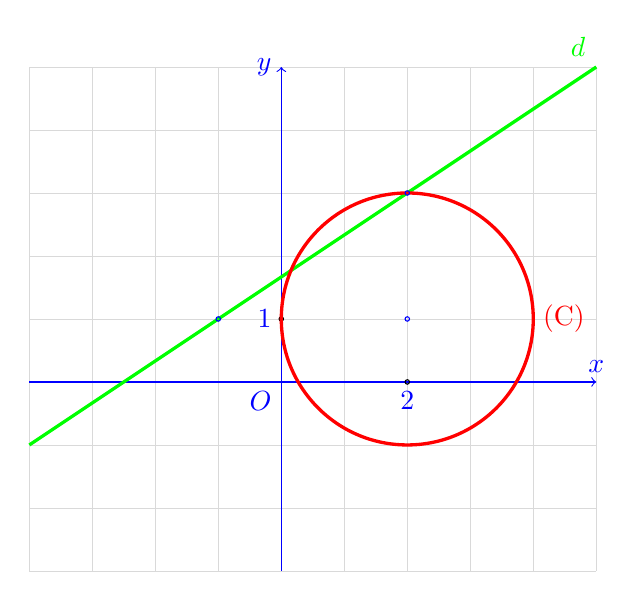
\begin{tikzpicture}[scale=0.8]
		\draw[step=1,gray, very thin,opacity=0.3](-4,-3) grid (5,5);
		\draw [->,blue] (-4,0) -- (5,0) node[above] {$x$};
		\draw [->,blue] (0,-3) -- (0,5) node[left] {$y$};
		\foreach \x in {2} {\draw (\x,0) node[below,blue] {$\x$} circle (1pt);}
		\foreach \y in {1} {\draw (0,\y) node[left,blue] {$\y$} circle (1pt);}
		\draw (0,0) node [below left,blue]{$O$};
		\draw[smooth,green, very thick] plot[domain=-4:5] (\x, {(2/3)*(\x) +(5/3)}) node[above left] {$d$};
		\draw[red, very thick] (2,1) circle (2) ;
		\draw (4,1) node [right,red] {(C)} ;
		\draw[blue] (-1,1) circle (1pt);
		\draw[blue] (2,3) circle (1pt);
		\draw[blue] (2,1) circle (1pt);
		\end{tikzpicture}\]
\loigiai{
	\begin{enumerate}[a)]
		\item Lập phương trình đường thẳng $d$;\\
		Dựa vào đồ thị hình 64, ta thấy đường thẳng $d$ đi qua hai điểm $A(-1;1)$ và $B(2;3)$.\\
		Phương trình tham số đường thẳng $d$ đi qua $A(-1;1)$ và có một vectơ chỉ phương là $\vec{u}=\vec{AB}=(3;2)$:\\
		\[d:\left\{ {\begin{array}{*{20}{c}}
		  {x =  - 1 + 3t} \\
		  {y = 1 + 2t}
		\end{array}} \right.\]
		$(t \in \mathbb{R})$.
		\item Lập phương trình đường tròn $(C)$;\\
		Phương trình đường tròn $(C)$ có tâm $I(2;1)$ và bán kính $R=2$:
				\[(C): (x-2)^2+(y-1)^2=4\]
		\item Lập phương trình tiếp tuyến của đường tròn $(C)$ tại điểm $M(2+\sqrt{2} ; 1+\sqrt{2})$.\\
		Gọi $d$ là tiếp tuyến của đường tròn $(C)$ tại điểm $M$. \\
		Khi đó $d$ và $IM$ vuông góc với nhau.\\
		Phương trình đường thẳng $d$ qua $M(2+\sqrt{2} ; 1+\sqrt{2})$ và $\overrightarrow{IM}=(\sqrt{2} ; \sqrt{2})$ là vectơ pháp tuyến:\\
		\[d: \sqrt{2}(x-2-\sqrt{2})+\sqrt{2}(y-1-\sqrt{2})=0\]
		\[d: (x-2-\sqrt{2})+(y-1-\sqrt{2})=0\]
		\[d: x+y-3-2\sqrt{2})=0\]
		\end{enumerate}
}
\end{bt}

\begin{bt}%[0H3B1-4]
	Cho hai đường thẳng
	$$
	\Delta_{1}: \sqrt{3} x+y-4=0, \Delta_{2}: x+\sqrt{3} y-2 \sqrt{3}=0 \text {. }
	$$
	\begin{enumerate}[a)]
	\item Tìm tọa độ giao điểm hai đường thẳng đã cho;
	\item Tính góc $\alpha$ giữa hai đường thẳng đã cho.
	\end{enumerate}
	\loigiai{
	\begin{enumerate}[a)]
		\item Tọa độ giao điểm hai đường thẳng đã cho là nghiệm của hệ phương trình:
		\[\left\{ {\begin{array}{*{20}{c}}
		  {\sqrt 3 x + y - 4 = 0} \\
		  {x + \sqrt 3 y - 2\sqrt 3  = 0{\text{ }}}
		\end{array} \Leftrightarrow } \right.\left\{ {\begin{array}{*{20}{c}}
		  {\sqrt 3 x + y = 4} \\
		  {x + \sqrt 3 y = 2\sqrt 3 {\text{ }}}
		\end{array}} \right. \Leftrightarrow \left\{ {\begin{array}{*{20}{c}}
		  {x = \sqrt 3 } \\
		  {y = 1}
		\end{array}} \right.\]
		Vậy $(\sqrt{3};1)$ tọa độ giao điểm hai đường thẳng đã cho.
		\item Tính góc $\alpha$ giữa hai đường thẳng đã cho.\
		\[\cos \left(\Delta_{1}, \Delta_{2}\right)=\left|\cos \left(\overrightarrow{n_{1}}, \overrightarrow{n_{2}}\right)\right|=\dfrac{\left|\overrightarrow{n_{1}} \cdot \overrightarrow{n_{2}}\right|}{\left|\overrightarrow{n_{1}}\right| \cdot\left|\overrightarrow{n_{2}}\right|} = \dfrac{{\left| {\sqrt 3 .1 + 1.\sqrt 3 } \right|}}{{\sqrt {3 + 1} .\sqrt {1 + 3} }} = \dfrac{{2\sqrt 3 }}{4} = \dfrac{{\sqrt 3 }}{2}.\]
		$\Rightarrow \left( {{\Delta _1},{\Delta _2}} \right) = {30^ \circ }.$
		\end{enumerate}
	}
\end{bt}

\begin{bt}%[0H3B3-1]
	Cho biết mỗi đường conic có phương trình dưới đây là đường conic dạng nào (elip, hypebol, parabol) và tìm toạ độ tiêu điểm của đường conic đó.
\begin{enumerate}[a)]
	\item $y^{2}=18 x$;
	\item $\dfrac{x^{2}}{64}+\dfrac{y^{2}}{25}=1$;
	\item $\dfrac{x^{2}}{9}-\dfrac{y^{2}}{16}=1$.
	\end{enumerate}
\loigiai{
\begin{enumerate}[a)]
	\item $y^{2}=18 x$ là đường conic dạng parabol vì có dạng $y^2=2px$ với $p=9>0$.\\
	Tọa độ tiêu điểm của parabol là $F\left(\dfrac{p}{2};0 \right)=F\left(\dfrac{9}{2};0 \right)$.
	\item $\dfrac{x^{2}}{64}+\dfrac{y^{2}}{25}=1$ là đường conic dạng elip vì có dạng $\dfrac{x^{2}}{a^2}+\dfrac{y^{2}}{b^2}=1$ với $a=8,b=5$ thỏa điều kiện $a>b>0$.\\
	Suy ra $c=\sqrt{a^2-b^2}=\sqrt{8^2-5^2}=\sqrt{39}$.\\
	Tọa độ hai tiêu điểm của elip là $F_1 \left(-c;0 \right)=F_1\left(-\sqrt{39};0 \right)$ và $F_2 \left(c;0 \right)=F_2 \left(\sqrt{39};0 \right)$.
	\item $\dfrac{x^{2}}{9}-\dfrac{y^{2}}{16}=1$ là đường conic dạng hypebol vì có dạng $\dfrac{x^{2}}{a^2}-\dfrac{y^{2}}{b^2}=1$ với $a=3,b=4$ thỏa điều kiện $a>0,b>0$.\\
	Suy ra $c=\sqrt{a^2+b^2}=\sqrt{3^2+4^2}=5$.\\
	Tọa độ hai tiêu điểm của elip là $F_1 \left(-c;0 \right)=F_1\left(-5;0 \right)$ và $F_2 \left(c;0 \right)=F_2 \left(5;0 \right)$.
	\end{enumerate}
}
\end{bt}

\begin{bt}%[0H3B3-2]
Cho tam giác $A F_{1} F_{2}$, trong đó $A(0 ; 4), F_{1}(-3 ; 0), F_{2}(3 ; 0)$.
\begin{enumerate}
\item Lập phương trình tổng quát của các đường thẳng $A F_{1}$ và $A F_{2}$.
\item Lập phương trình đường tròn ngoại tiếp của tam giác $A F_{1} F_{2}$.
\item Lập phương trình chính tắc của elip $(E)$ có hai tiêu điểm là $F_{1}, F_{2}$ sao cho $(E)$ đi qua $A$.
\end{enumerate}
\loigiai{
\begin{enumerate}
\item \textit{Lập phương trình tổng quát của các đường thẳng $A F_{1}$.}\\
Ta có: Một vectơ chỉ phương của $AF_1$ là $\vec{u}=\vec{AF_1}=(-3;-4)$.\\
Suy ra một vectơ pháp tuyến của $AF_1$ là $\vec{n}=(4;-3)$.\\
Phương trình tổng quát đường thẳng $AF_1$ qua điểm $A(0;4)$ và có một vectơ pháp tuyến $\vec{n}=(4;-3)$:\\
\[d: 4(x-0)-3(y-4)=0\]
\[d: 4x-3y+12=0\]
\textit{Lập phương trình tổng quát của các đường thẳng $A F_{2}$.}\\
Ta có: Một vectơ chỉ phương của $AF_2$ là $\vec{u}=\vec{AF_2}=(3;-4)$.\\
Suy ra một vectơ pháp tuyến của $AF_2$ là $\vec{n}=(4;3)$.\\
Phương trình tổng quát đường thẳng $AF_2$ qua điểm $A(0;4)$ và có một vectơ pháp tuyến $\vec{n}=(4;3)$:\\
\[d: 4(x-0)+3(y-4)=0\]
\[d: 4x+3y-12=0\]
\item Lập phương trình đường tròn ngoại tiếp của tam giác $A F_{1} F_{2}$.\\
Phương trình đường tròn $(C)$ ngoại tiếp tam giác $AF_1F_2$ có dạng\\
	\[(C): x^2+y^2-2ax-2by+c=0\]
	có tâm $I(a;b)$ và bán kính $R=\sqrt{a^2+b^2-c}$.\\
	Ta có
	\[\left\{ {\begin{array}{*{20}{c}}
	  {A( 0;4) \in (C)} \\
	  {F_1( - 3; 0) \in (C)} \\
	  {F_2(3;0) \in (C)}
	\end{array}} \right. \Rightarrow \left\{ {\begin{array}{*{20}{c}}
	  { {4^2} - 8b + c = 0} \\
	  {{{( - 3)}^2} + 6a + c = 0} \\
	  {{3^2} - 6a + c = 0}
	\end{array}} \right.\]
	\[ \Rightarrow \left\{ {\begin{array}{*{20}{c}}
	  {- 8b + c =  - 16} \\
	  {6a + c =  - 9} \\
	  { -6a  + c =  - 9}
	\end{array} \Rightarrow \left\{ {\begin{array}{*{20}{c}}
	  {a = 0} \\
	  {b =  \dfrac{7}{8}} \\
	  {c =  - 9}
	\end{array}} \right.} \right.\]
	Phương trình đường tròn $(C)$ có tâm $I(0 ; \dfrac{7}{8})$ và bán kính\\ $R=\sqrt{0^2+ \left( \dfrac{7}{8}\right) ^2+9}= \dfrac{25}{8}$:
		\[(C): x^2+(y- \dfrac{7}{8})^2= \dfrac{625}{64}\]
\item Lập phương trình chính tắc của elip $(E)$ có hai tiêu điểm là $F_{1}, F_{2}$ sao cho $(E)$ đi qua $A$.\\
	Phương trình chính tắc của elip $(E)$ có dạng $\dfrac{x^{2}}{a^2}+\dfrac{y^{2}}{b^2}=1$ thỏa điều kiện $a>b>0$.\\
	Vì $(E)$ đi qua $A(0;4)$ nên $\dfrac{0^{2}}{a^2}+\dfrac{4^{2}}{b^2}=1 \Leftrightarrow \dfrac{4^{2}}{b^2}=1 \Leftrightarrow b^2=4^2 \Leftrightarrow b= 4.$ (do $b>0 $)\\
	Suy ra $a=\sqrt{c^2+b^2}=\sqrt{3^2+4^2}=5$.\\
	Vậy phương trình chính tắc của elip $(E)$ có dạng $\dfrac{x^{2}}{25}+\dfrac{y^{2}}{4}=1$.
\end{enumerate}
}
\end{bt}
\begin{bt}%[0H3T1-7]
Trên màn hình ra-đa của đài kiểm soát không lưu sân bay $A$ có hệ trục toạ độ $Oxy$ (Hình 65), trong đó đơn vị trên mỗi trục tính theo ki-lô-mét và đài kiểm soát được coi là gốc toạ độ $O(0 ; 0)$. Nếu máy bay bay trong phạm vi cách đài kiểm soát $500 \mathrm{~km}$ thì sẽ hiển thị trên màn hình ra-đa.\\
Một máy bay khởi hành từ sân bay $B$ lúc 14 giờ. Sau thời gian $t$ (giờ), vị trí của máy bay được xác định bởi điểm $M$ có toạ độ như sau:
\[\left\{ {\begin{array}{*{50}{c}}
  {x = \dfrac{{1600}}{3} - \dfrac{{1400}}{3}t} \\
  {y = \dfrac{{1900}}{3} - \dfrac{{1400}}{3}t}
\end{array}} \right.\]
\begin{enumerate}
\item Tìm vị trí của máy bay lúc 14 giờ 30 phút. Thời điểm này máy bay đã xuất hiện trên màn hình ra-đa chưa?
\item Lúc mấy giờ máy bay bay gần đài kiểm soát không lưu nhất? Tính khoảng cách giữa máy bay và đài kiểm soát không lưu lúc đó.
\item Máy bay ra khỏi màn hình ra-đa vào thời gian nào?
\end{enumerate}
\loigiai{
\begin{enumerate}
\item Tìm vị trí của máy bay lúc 14 giờ 30 phút. Thời điểm này máy bay đã xuất hiện trên màn hình ra-đa chưa?\\
Lúc 14 giờ 30 phút, máy bay đã khởi hành được $30$ phút $= \dfrac{1}{2}$ giờ.\\
Khi đó vị trí của máy bay là điểm $N(x_N;y_N)$ có tọa độ
\[\left\{ {\begin{array}{*{20}{c}}
  {{x_N} = \dfrac{{1600}}{3} - \dfrac{{1400}}{3}.\dfrac{1}{2} = 300} \\
  {{y_N} = \dfrac{{1900}}{3} - \dfrac{{1400}}{3}.\dfrac{1}{2} = 400}
\end{array}} \right.\]
Do $x_N=300<500$ và $y_N=400<500$ nên ở thời điểm này máy bay đã xuất hiện trên màn hình ra-đa.
\item Lúc mấy giờ máy bay bay gần đài kiểm soát không lưu nhất? Tính khoảng cách giữa máy bay và đài kiểm soát không lưu lúc đó.\\
Khi máy bay gần đài kiểm soát nhất thì tọa độ của máy bay giả sử là điểm $P\left( \dfrac{{1600}}{3} - \dfrac{{1400}}{3}.t; \dfrac{{1900}}{3} - \dfrac{{1400}}{3}.t \right) $ gần sát với tọa độ của đài kiểm soát là điểm $O$, tức ta có độ dài đoạn thẳng $OP$ nhỏ nhất.\\
Ta tính được \\
$OP^2= \left( \dfrac{{1600}}{3} - \dfrac{{1400}}{3}.t\right) ^2+\left(\dfrac{{1900}}{3} - \dfrac{{1400}}{3}.t \right) ^2 $\\
$ = \dfrac{{3920000}}{9}t^2 - \dfrac{{9800000}}{9}.t+\dfrac{6170000}{9}$ \\
$ = \dfrac{{3920000}}{9}\left( t^2 - \dfrac{{5}}{2}t\right) +\dfrac{6170000}{9}$ \\
$ = \dfrac{{3920000}}{9}\left( t^2 - \dfrac{{5}}{2}t+\dfrac{25}{16}\right) +500$ \\
$ = \dfrac{{3920000}}{9}\left( t - \dfrac{5}{4}\right)^2 +5000 \geq 5000$ \\
Dấu bằng xảy ra khi và chỉ khi $\left( t - \dfrac{5}{4}\right)^2=0 \Leftrightarrow t=\dfrac{5}{4}$.\\
Vậy lúc $15$ giờ $15$ phút thì máy bay gần đài kiểm soát không lưu nhất. Khoảng cách giữa máy bay và đài kiểm soát lúc đó là $50\sqrt{2}\;$ km.
\item Máy bay ra khỏi màn hình ra-đa vào thời gian nào?\\
Khi máy bay ra khỏi màn hình ra-đa thì tọa độ của máy bay giả sử là điểm $Q\left( \dfrac{{1600}}{3} - \dfrac{{1400}}{3}.t; \dfrac{{1900}}{3} - \dfrac{{1400}}{3}.t \right) $ cách tọa độ của đài kiểm soát là điểm $O$ hơn $500$, tức ta có độ dài đoạn thẳng $OQ>500$.\\
Ta có $OQ>500 \Leftrightarrow OQ^2 > 250000$\\
$ \Leftrightarrow \left( \dfrac{{1600}}{3} - \dfrac{{1400}}{3}.t\right) ^2+\left(\dfrac{{1900}}{3} - \dfrac{{1400}}{3}.t \right) ^2 >250000$ \\
$ \Leftrightarrow \dfrac{{3920000}}{9}t^2 - \dfrac{{9800000}}{9}.t+\dfrac{3920000}{9}>0$ \\
$ \Leftrightarrow t^2 - \dfrac{{5}}{2}.t+1>0$ \\
$ \Leftrightarrow t<\dfrac{1}{2} \text{hoặc} t>2$.\\
Vậy máy bay ra khỏi màn hình ra-đa vào lúc $16$ giờ.
\end{enumerate}
}
\end{bt}
%\subsection{BÀI TẬP TRONG SÁCH KẾT NỐI}
%\subsubsection{TRẮC NGHIỆM}
%\subsubsection{TỰ LUẬN}
\setcounter{bt}{0}
\begin{bt}%[0H3K1-4]
Trong mặt phẳng tọa độ, cho $A(1 ;-1), B(3 ; 5), C(-2 ; 4)$. Tính diện tích tam giác $ABC$.
\loigiai{
Ta có
$$\begin{aligned}
&\overrightarrow{A B}=\left(x_{B}-x_{A} ; y_{B}-y_{A}\right)=\left(2 ; 6\right) \Rightarrow A B=\sqrt{2^{2}+6^{2}}=2\sqrt{10}.\\
&\overrightarrow{A C}=\left(x_{C}-x_{A} ; y_{C}-y_{A}\right)=\left(-3 ; 5\right) \Rightarrow A C=\sqrt{(-3)^{2}+ 5^{2}}=\sqrt{34}.\\
&\cos \widehat{B A C}=\cos (\overrightarrow{A B}, \overrightarrow{A C})=\dfrac{2. (-3)+6.5}{\sqrt{2^{2}+6^{2}} \sqrt{(-3)^{2}+5^{2}}}=\\
&\text { Do } \sin \widehat{B A C}>0 \text { nên }\\
&\sin \widehat{B A C}=\sqrt{1-\cos ^{2}\widehat{B A C}}=\sqrt{1-\left(\dfrac{2. (-3)+6.5}{\sqrt{2^{2}+6^{2}} \sqrt{(-3)^{2}+5^{2}}}\right)^{2}}\\
&=\dfrac{\left|2.5-(-3). 6\right|}{\sqrt{2^{2}+6^{2}} \sqrt{(-3)^{2}+5^{2}}}
\end{aligned}$$
Suy ra
$$S_{\triangle A B O}=\dfrac{1}{2} A B \cdot A C \cdot \sin \widehat{B A C}=\dfrac{1}{2}\left|2.5-(-3). 6\right|=14 \text{(đvdt)}.$$
}
\end{bt}
\begin{bt}%[0H3B2-2]
Trong mặt phẳng toạ độ, cho hai điểm $A(-1 ; 0)$ và $B(3 ; 1)$.
\begin{enumerate}[a)]
\item Viết phương trình đường tròn tâm $A$ và đi qua $B$.
\item Viết phương trình tồng quát của đường thẳng $A B$.
\item Viết phương trình đường tròn tâm $O$ và tiếp xúc với đường thẳng $AB$.
\end{enumerate}
\loigiai{
\begin{enumerate}[a)]
\item Viết phương trình đường tròn tâm $A$ và đi qua $B$.\\
Phương trình đường tròn $(C)$ có tâm $A(-1 ; 0)$ và bán kính\\ $R=AB=\sqrt{(3+1)^2+(1-0)^2}=\sqrt{17}$:
		\[(C): (x+1)^2+y^2=17\]
\item Viết phương trình tổng quát của đường thẳng $AB$.\\
		Ta có $\vec{AB}=(4;1)$.\\
		Phương trình tổng quát $AB$ đi qua điểm $A(-1 ;0)$ và có một vectơ pháp tuyến là $\vec{n}=(1 ; -4)$:\\
		\[d: 1(x+1)-4(y-0)=0\]
		\[d: x-4y+1=0\]
\item Viết phương trình đường tròn tâm $O$ và tiếp xúc với đường thẳng $AB$.\\
	Ta có $d(O,AB)=\dfrac{\left| 0 -4.0+1 \right|}{\sqrt{1^2+(-4)^2}}=\dfrac{\sqrt{17}}{17}$.\\
	Phương trình đường tròn tâm $O(0;0)$ có bán kính $R=d(O,AB)=\dfrac{\sqrt{17}}{17}$:\\
	\[(C): (x-0)^2+(y-0)^2=\dfrac{1}{17}\]
	\[(C): x^2+y^2=\dfrac{1}{17}\]
\end{enumerate}
}
\end{bt}

\begin{bt}%[0H3B2-3]
Cho đường tròn $(C)$ có phương trình $x^{2}+y^{2}-4 x+6 y-12=0$.
\begin{enumerate}[a)]
\item Tìm toạ độ tâm và bán kính $R$ của $(C)$.
\item Chứng minh rằng điểm $M(5 ; 1)$ thuộc $(C)$. Viết phương trình tiếp tuyến $d$ của $(C)$ tại $M$.
\end{enumerate}
\loigiai{
\begin{enumerate}[a)]
\item Tìm toạ độ tâm và bán kính $R$ của $(C)$.\\
Từ phương trình $(C): x^{2}+y^{2}-4 x+6 y-12=0$ ta suy ra $a=\dfrac{-4}{-2}=2, b=\dfrac{6}{-2}=-3, c=-12$.\\
Khi đó $R=\sqrt{a^2+b^2-c}=\sqrt{2^2+(-3)^2+12}=5$.\\
Vậy $(C)$ có tâm $I(2;-3) $ và có bán kính $R=5$.
\item Chứng minh rằng điểm $M(5 ; 1)$ thuộc $(C)$. Viết phương trình tiếp tuyến $d$ của $(C)$ tại $M$.\\
Thay tọa độ điểm $M(5 ; 1)$ vào $(C): x^{2}+y^{2}-4 x+6 y-12=0$ ta được\\
\[5^{2}+1^{2}-4.5+6.1-12=0\]
\[0=0 \; \text{(luôn đúng)}.\]
Vậy $M(5 ; 1)$ thuộc $(C)$.\\
Gọi $d$ là tiếp tuyến của đường tròn $(C)$ tại điểm $M$. \\
Khi đó $d$ và $IM$ vuông góc với nhau.\\
Phương trình đường thẳng $d$ qua $M(5 ; 1)$ và $\overrightarrow{IM}=(3 ; 4)$ là vectơ pháp tuyến:\\
		\[d: 3(x-5)+4(y-1)=0\]
		\[d: 3x+4y-19=0\]
\end{enumerate}
}
\end{bt}

\begin{bt}%[0H3K3-3]
Cho elip $(E): \dfrac{x^{2}}{a^{2}}+\dfrac{y^{2}}{b^{2}}=1 \; (a>b>0)$.
\begin{enumerate}[a)]
\item Tìm các giao điểm $A_{1}, A_{2}$ của $(E)$ với trục hoành và các giao điểm $B_{1}, B_{2}$ của $(E)$ với trục tung. Tính $A_{1} A_{2}, B_{1} B_{2}$.
\item Xét một điểm bất kì $M\left(x_{0}, y_{0}\right)$ thuộc $(E)$.
Chứng minh rằng, $b^{2} \leq x_{0}^{2}+y_{0}^{2} \leq a^{2}$ và $b \leq O M \leq a$.\\
\textbf{Chú ý.} $A_{1} A_{2}, B_{1} B_{2}$ tương ứng được gọi là trục lớn, trục nhỏ của elip $(E)$ và tương ứng có độ dài là $2 a, 2 b$.
\end{enumerate}
\loigiai{
\begin{enumerate}[a)]
\item
\textit{Giao điểm của $(E)$ với trục hoành:}\\
$$\dfrac{x^{2}}{a^{2}}+\dfrac{0^{2}}{b^{2}}=1 $$
$$\Leftrightarrow \dfrac{x^{2}}{a^{2}}=1 $$
$$\Leftrightarrow x^{2}=a^{2} $$
$$\Leftrightarrow x=\pm a $$
Vậy $A_1(a;0),A_2(-a;0)$ là giao điểm của $(E)$ với trục hoành.\\
\textit{Giao điểm của $(E)$ với trục tung:}\\
$$\dfrac{0^{2}}{a^{2}}+\dfrac{y^{2}}{b^{2}}=1 $$
$$\Leftrightarrow \dfrac{y^{2}}{b^{2}}=1 $$
$$\Leftrightarrow y^{2}=b^{2} $$
$$\Leftrightarrow y=\pm b $$
Vậy $B_1(0;b),B_2(0;-b)$ là giao điểm của $(E)$ với trục tung.\\
Ta có $A_1A_2=\sqrt{(-a-a)^2+(0-0)^2}=2a.$\\
$B_1B_2=\sqrt{(0-0)^2+(-b-b)^2}=2b.$
\item Xét một điểm bất kì $M\left(x_{0}, y_{0}\right)$ thuộc $(E)$.
Chứng minh rằng, $b^{2} \leq x_{0}^{2}+y_{0}^{2} \leq a^{2}$ và $b \leq O M \leq a$.\\
\textit{Chứng minh $x_0^2+y_0^2 \geq b^2$.}\\
Vì $M\left(x_{0}, y_{0}\right)$ thuộc $(E)$ nên ta có
$$\dfrac{x_0^{2}}{a^{2}}+\dfrac{y_0^{2}}{b^{2}}=1 $$
Suy ra $y_0^2=b^2.\left( 1- \dfrac{x_0^{2}}{a^{2}} \right) $.\\
Thay $y_0^2$ vừa tìm được vào $x_{0}^{2}+y_{0}^{2}$:
$$x_{0}^{2}+y_{0}^{2}= x_{0}^{2}+ b^2.\left( 1- \dfrac{x_0^{2}}{a^{2}} \right)$$
$$ =b^2 +x_0^2.\left( 1 - \dfrac{b^2}{a^2}\right)  $$
$$ =b^2 +x_0^2.\left( \dfrac{a^2-b^2}{a^2}\right) $$
Vì theo giả thiết $a>b>0$ nên $a^2>b^2>0$. Suy ra $a^2-b^2 >0$. \\
Suy ra $\dfrac{a^2-b^2}{a^2} >0$.\\
Mặt khác $x_0^2 \geq 0$ nên $x_0^2.\left( \dfrac{a^2-b^2}{a^2}\right) \geq 0$.\\
Do đó $b^2 +x_0^2.\left( \dfrac{a^2-b^2}{a^2}\right) \geq b^2$, tức $x_{0}^{2}+y_{0}^{2} \geq b^2.$\\
Dấu bằng xảy ra khi \[\left\{ {\begin{array}{*{20}{c}}
  {{x_0} = 0} \\
  {y_0^2 = {b^2}.\left( {1 - \dfrac{{x_0^2}}{{{a^2}}}} \right)}
\end{array}} \right. \Leftrightarrow \left\{ {\begin{array}{*{20}{c}}
  {{x_0} = 0} \\
  {y_0^2 = {b^2}}
\end{array}} \right. \Leftrightarrow \left\{ {\begin{array}{*{20}{c}}
  {{x_0} = 0} \\
  {{y_0} =  \pm b}
\end{array}} \right.\]

\textit{Chứng minh $x_0^2+y_0^2 \leq a^2$.}\\
Vì $M\left(x_{0}, y_{0}\right)$ thuộc $(E)$ nên ta có
$$\dfrac{x_0^{2}}{a^{2}}+\dfrac{y_0^{2}}{b^{2}}=1 $$
Suy ra $x_0^2=a^2.\left( 1- \dfrac{y_0^{2}}{b^{2}} \right) $.\\
Thay $x_0^2$ vừa tìm được vào $x_{0}^{2}+y_{0}^{2}$:
$$x_{0}^{2}+y_{0}^{2}=a^2.\left( 1- \dfrac{y_0^{2}}{b^{2}} \right) + y_{0}^{2} $$
$$ =a^2 +y_0^2.\left( 1 - \dfrac{a^2}{b^2}\right)  $$
$$ =a^2 +y_0^2.\left( \dfrac{b^2-a^2}{b^2}\right) $$
Vì theo giả thiết $a>b>0$ nên $a^2>b^2>0$. Suy ra $a^2-b^2 >0$ hay $b^2-a^2 <0$. \\
Suy ra $\dfrac{b^2-a^2}{a^2} <0$.\\
Mặt khác $y_0^2 \geq 0$ nên $y_0^2.\left( \dfrac{b^2-a^2}{b^2}\right) \leq 0$.\\
Do đó $a^2 +y_0^2.\left( 1 - \dfrac{a^2}{b^2}\right) \leq a^2$, tức $x_{0}^{2}+y_{0}^{2} \leq a^2.$\\
Dấu bằng xảy ra khi \[\left\{ {\begin{array}{*{20}{c}}
  {{y_0} = 0} \\
  {x_0^2 = a^2 +y_0^2.\left( \dfrac{b^2-a^2}{b^2}\right)}
\end{array}} \right. \Leftrightarrow \left\{ {\begin{array}{*{20}{c}}
  {{y_0} = 0} \\
  {x_0^2 = {a^2}}
\end{array}} \right. \Leftrightarrow \left\{ {\begin{array}{*{20}{c}}
  {{y_0} = 0} \\
  {{x_0} =  \pm a}
\end{array}} \right.\]
Vậy ta đã chứng minh được $b^{2} \leq x_{0}^{2}+y_{0}^{2} \leq a^{2}$.\\
\textit{Chứng minh $b \leq O M \leq a$.}\\
Ta có
\[OM=\sqrt{x_0^2+y_0^2}\]
Ở chứng minh trên, ta đã chứng minh
$b^{2} \leq x_{0}^{2}+y_{0}^{2} \leq a^{2}$.\\
Điều này tương đương với
\[b \leq \sqrt{x_0^2+y_0^2} \leq a\]
\[\Leftrightarrow b \leq \sqrt{x_0^2+y_0^2} \leq a\]
\[\Leftrightarrow b \leq OM \leq a \; \text{đpcm.}\]
\end{enumerate}
}
\end{bt}

\begin{bt}%[0H3K3-3]
Cho hypebol có phương trình: $\dfrac{x^{2}}{a^{2}}-\dfrac{y^{2}}{b^{2}}=1$.
\begin{enumerate}[a)]
\item Tìm các giao điểm $A_{1}, A_{2}$ của hypebol với trục hoành (hoành độ của $A_{1}$ nhỏ hơn của $A_{2}$ ).
\item Chứng minh rằng, nếu điểm $M(x ; y)$ thuộc nhánh nằm bên trái trục tung của hypebol thì $x \leq-a$, nếu điểm $M(x ; y)$ thuộc nhánh nằm bên phải trục tung của hypebol thì $x \geq a$.
\item Tìm các điểm $M_{1}, M_{2}$ tương ứng thuộc các nhánh bên trái, bên phải trục tung của hypebol để $M_{1} M_{2}$ nhỏ nhất.
\end{enumerate}
\loigiai{
\begin{enumerate}[a)]
\item Tìm các giao điểm $A_{1}, A_{2}$ của hypebol với trục hoành (hoành độ của $A_{1}$ nhỏ hơn của $A_{2}$ ).\\
\textit{Giao điểm của hypebol $(H)$ với trục hoành:}\\
$$\dfrac{x^{2}}{a^{2}}-\dfrac{0^{2}}{b^{2}}=1 $$
$$\Leftrightarrow \dfrac{x^{2}}{a^{2}}=1 $$
$$\Leftrightarrow x^{2}=a^{2} $$
$$\Leftrightarrow x=\pm a $$
Vậy $A_1(-a;0),A_2(a;0)$ là giao điểm của $(H)$ với trục hoành (vì hoành độ của $A_{1}$ nhỏ hơn của $A_{2}$ ).
\item
\textit{Chứng minh rằng, nếu điểm $M(x ; y)$ thuộc nhánh nằm bên trái trục tung của hypebol thì $x \leq-a$.}\\
Vì $M\left(x, y\right)$ thuộc $(H)$ nên ta có
$$\dfrac{x^{2}}{a^{2}}-\dfrac{y^2}{b^{2}}=1$$
Suy ra $x^2=a^2.\left( 1+ \dfrac{y^{2}}{b^{2}} \right) \Leftrightarrow |x|=|a|.\sqrt{\left( 1+ \dfrac{y^{2}}{b^{2}} \right)} \Leftrightarrow x=-a.\sqrt{\left( 1+ \dfrac{y^{2}}{b^{2}} \right)}$\\
(vì $M(x;y)$ thuộc nhánh bên trái trục tung của $(H)$ nên $x<0$.)\\
Hơn nữa, ta có $\sqrt{\left( 1+ \dfrac{y^{2}}{b^{2}} \right)} \geq 1$ nên $-a.\sqrt{\left( 1+ \dfrac{y^{2}}{b^{2}} \right)} \leq -a$ hay $x \leq -a$.\\
\textit{Chứng minh rằng, nếu điểm $M(x ; y)$ thuộc nhánh nằm bên phải trục tung của hypebol thì $x \geq a$.}\\
Vì $M\left(x, y\right)$ thuộc $(H)$ nên ta có
$$\dfrac{x^{2}}{a^{2}}-\dfrac{y^2}{b^{2}}=1$$
Suy ra $x^2=a^2.\left( 1+ \dfrac{y^{2}}{b^{2}} \right) \Leftrightarrow |x|=|a|.\sqrt{\left( 1+ \dfrac{y^{2}}{b^{2}} \right)} \Leftrightarrow x=a.\sqrt{\left( 1+ \dfrac{y^{2}}{b^{2}} \right)}$\\
(vì $M(x;y)$ thuộc nhánh bên phải trục tung của $(H)$ nên $x>0$.)\\
Hơn nữa, ta có $\sqrt{\left( 1+ \dfrac{y^{2}}{b^{2}} \right)} \geq 1$ nên $a.\sqrt{\left( 1+ \dfrac{y^{2}}{b^{2}} \right)} \geq a$ hay $x \geq a$.\\
\item Tìm các điểm $M_{1}, M_{2}$ tương ứng thuộc các nhánh bên trái, bên phải trục tung của hypebol để $M_{1} M_{2}$ nhỏ nhất.\\
Gọi $M_1(x_1;y_1), M_2(x_2;y_2)$.\\
Vì $M_1$ thuộc nhánh bên trái của $(H)$ nên $x_1=-a.\sqrt{\left( 1+ \dfrac{y_1^{2}}{b^{2}} \right)}.$\\
Vì $M_2$ thuộc nhánh bên phải của $(H)$ nên $x_2=a.\sqrt{\left( 1+ \dfrac{y_2^{2}}{b^{2}} \right)}.$\\
Khi đó ${M_1M_2}^2= (x_2-x_1)^2+(y_2-y_1)^2=\left( a.\sqrt{1+ \dfrac{y_2^{2}}{b^{2}}} + a.\sqrt{1+ \dfrac{y_1^{2}}{b^{2}}}\right)^2+(y_2-y_1)^2.$\\
$=a^2.\left( \sqrt{1+ \dfrac{y_2^{2}}{b^{2}}} + \sqrt{1+ \dfrac{y_1^{2}}{b^{2}}}\right)^2+(y_2-y_1)^2$.\\
Do $(y_2-y_1)^2 \geq 0$, $a^2>0$, $\dfrac{y_2^{2}}{b^{2}}, \dfrac{y_1^{2}}{b^{2}} \geq 0$ nên ${M_1M_2}$ nhỏ nhất khi và chỉ khi \[\left\{ {\begin{array}{*{20}{c}}
  {{{({y_2} - {y_1})}^2} = 0} \\
  {\dfrac{{y_1^2}}{{{b^2}}} = 0} \\
  {\dfrac{{y_2^2}}{{{b^2}}} = 0}
\end{array}} \right. \Leftrightarrow \left\{ {\begin{array}{*{20}{c}}
  {{y_2} = {y_1}} \\
  {{y_1} = 0} \\
  {{y_2} = 0}
\end{array}} \right. \Leftrightarrow {y_1} = {y_2} = 0\]
Khi đó $M_1M_2$ có độ dài nhỏ nhất là $=\sqrt{a^2.\left( \sqrt{1} + \sqrt{1}\right)^2}=2a$\\
trong đó $M_1(-a;0) \equiv A_1 , M_2(a;0) \equiv A_2.$
\end{enumerate}
}
\end{bt}

\begin{bt}%[0H3T3-4]
Một cột trụ hình hypebol (H.7.36), có chiều cao $6$ m, chỗ nhỏ nhất ở chính giữa và rộng $0,8$ m, đỉnh cột và đáy cột đều rộng $1$ m. Tính độ rộng của cột ở độ cao $5$ m (tính theo đơn vị mét và làm tròn tới hai chữ số sau dấu phầy).
	\[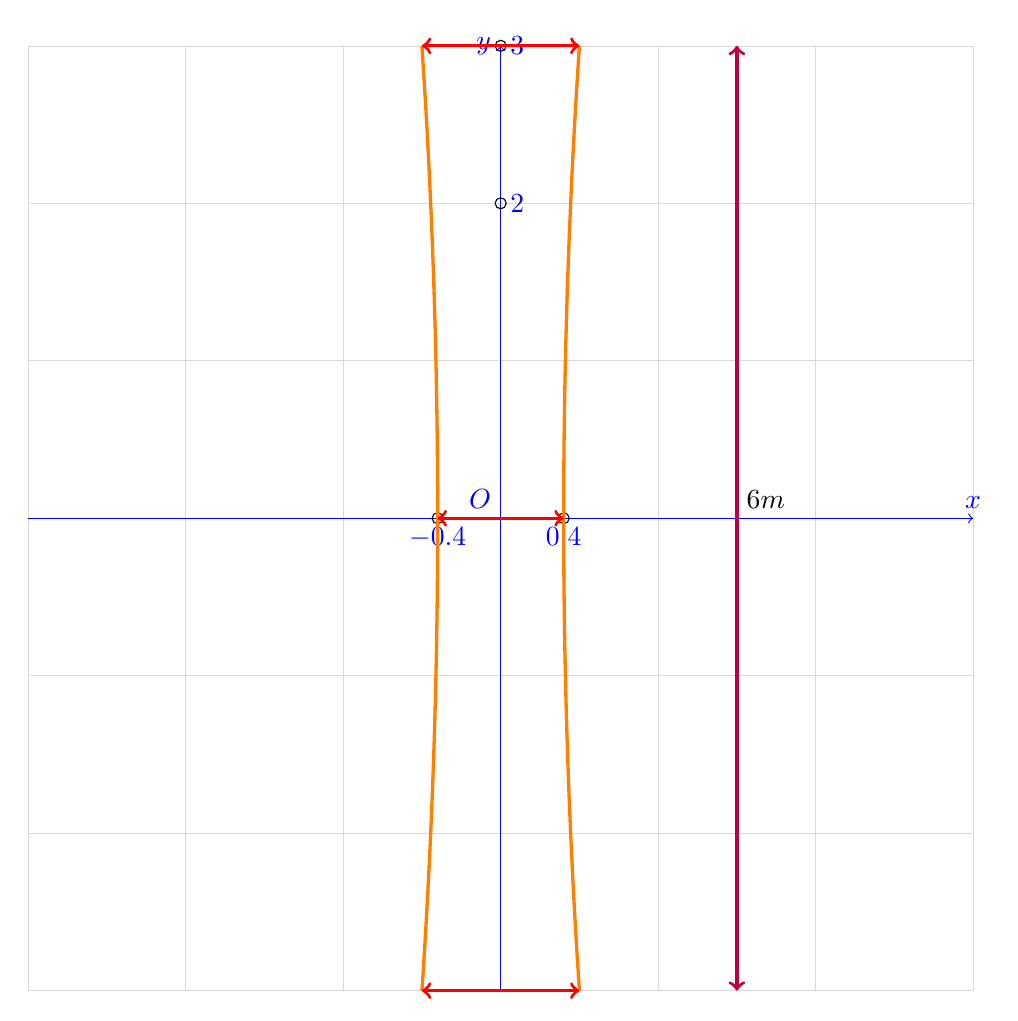
\begin{tikzpicture}[scale=2]
			\draw[step=1,gray, very thin,opacity=0.3](-3,-3) grid (3,3);
			\draw [->,blue] (-3,0) -- (3,0) node[above] {$x$};
			\draw [->,blue] (0,-3) -- (0,3) node[left] {$y$};
			\foreach \x in {-0.4,0.4} {\draw (\x,0) node[below,blue] {$\x$} circle (1pt);}
			\foreach \y in {2,3} {\draw (0,\y) node[right,blue] {$\y$} circle (1pt);}
			\draw (0,0) node [above left,blue]{$O$};
			\draw[smooth,orange, very thick] plot[domain=-3:3] ({(1/90)*(\x)^2+(2/5)}, \x);
			\draw[smooth,orange, very thick] plot[domain=-3:3] ({(-1/90)*(\x)^2-(2/5)}, \x);
			\draw[<->,red,very thick] (-0.4,0) -- (0.4,0);
			\draw[<->,red,very thick] (-0.5,3) -- (0.5,3);
			\draw[<->,red,very thick] (-0.5,-3) -- (0.5,-3);
			\draw[<->,purple,very thick] (1.5,-3) -- (1.5,3);
			\draw (1.5,0) node[above right] {$6 \text{m}$};
			\end{tikzpicture}\]
\loigiai{
Gắn hệ trục tọa độ $Oxy$ vào cột trụ hình Hypebol đã cho như hình trên.\\
Tiếp theo ta tìm phương trình của cột trụ hình Hypebol này.\\
Gọi phương trình của cột trụ là
$$\dfrac{x^{2}}{a^{2}}-\dfrac{y^{2}}{b^{2}}=1$$
Vì $Oy$ là đường trung trực của đoạn thẳng $0,8$ m nên $Oy$ chia đoạn thẳng $0,8$ m thành hai đoạn bằng nhau, mỗi đoạn $0,4$ m, tức Hypebol đi qua hai điểm $A_1(-0,4;0), A_2(0,4;0)$.\\
Khi đó ta có
$$\dfrac{{0,4}^{2}}{a^{2}}-\dfrac{0^{2}}{b^{2}}=1$$
$$\Leftrightarrow \dfrac{{0,4}^{2}}{a^{2}}=1$$
$$\Leftrightarrow a=0,4.$$
(vì $a>0$)\\
Lúc này ta được phương trình Hypebol: $$\dfrac{x^{2}}{0,16}-\dfrac{y^{2}}{b^{2}}=1$$
Vì $Oy$ là đường trung trực của đoạn thẳng $1$ m nên $Oy$ chia đoạn thẳng $1$ m thành hai đoạn bằng nhau, mỗi đoạn $0,5$ m, tức Hypebol đi qua hai điểm $B_1(-0,5;3), B_2(0,5;3)$.\\
Khi đó ta có
$$\dfrac{{0,5}^{2}}{0,16}-\dfrac{3^{2}}{b^{2}}=1$$
$$\Leftrightarrow \dfrac{3^{2}}{b^{2}}=\dfrac{9}{16}$$
$$\Leftrightarrow b=4.$$
(vì $b>0$)\\
Vậy ta đã tìm được phương trình Hypebol của cột trụ:
$$\dfrac{x^{2}}{0,16}-\dfrac{y^{2}}{16}=1$$
Khi cột trụ ở độ cao $5$ m thì
$$\dfrac{x^{2}}{0,16}-\dfrac{5^{2}}{16}=1$$
$$\Leftrightarrow \dfrac{x^{2}}{0,16}=\dfrac{41}{16}$$
$$\Leftrightarrow x^{2}=\dfrac{41}{100}$$
$$\Leftrightarrow |x|=\dfrac{\sqrt{41}}{10}$$
Vậy độ rộng của cột ở độ cao $5$ m là $2.|x|=2.\dfrac{\sqrt{41}}{10}=\dfrac{\sqrt{41}}{5} \approx 1,28 \;$ m.
}
\end{bt}
\Closesolutionfile{ans}